\documentclass[12pt, a4paper]{article}
%=========================== PACKAGES =============================%

\usepackage[utf8]{inputenc} 
\DeclareUnicodeCharacter{00A0}{ }

\usepackage[hmargin=1.5cm,vmargin=1.5cm]{geometry}
\usepackage[brazil]{babel}

\usepackage{longtable}
  
\usepackage{graphicx}
\usepackage{placeins}
\usepackage{subcaption}
\usepackage{float} 

\usepackage{hhline}
\usepackage{courier} 
 
\usepackage{amsmath}
\usepackage{bm}
\usepackage{amsfonts}

\usepackage[hyphens]{url}

\usepackage{listings}
\renewcommand\lstlistingname{Programa}
 
 
\usepackage{color} %red, green, blue, yellow, cyan, magenta, black, white
\lstset{language=bash,%
    basicstyle=\footnotesize\ttfamily,
    breaklines=true,%
    keywordstyle=[4]{\color{black}},
    frame= single,
}
 
\lstdefinestyle{nonumbers}
{numbers=none} 

\usepackage{multirow}

\usepackage{float}

\usepackage{enumerate}

\begin{document}

%    \maketitle
    {\large
    \centerline{\textbf{Relatório Exercício Prático 6}}
    \centerline{Gustavo Ciotto Pinton 117136}
    \centerline{EA979 - Processamento de Imagens}
    }

\section {Explicação}

A biblioteca \textit{OpenGL} utiliza, em seu processamento, um modelo contendo
duas pilhas de matrizes, chamadas de \textit{model-view} e \textit{projection},
sendo que, após a inicialização da aplicação, cada pilha contém apenas uma
matriz identidade. Tais matrizes representam um sistema de coordenadas
normalizadas, chamadas, em inglês, de \textit{normalized device coordinates},
cujos eixos X, Y e Z variam no intervalo de [-1,1]. A fim de mapear tais
eixos em coordenadas da janela de visualização, é necessário aplicarmos a
transformação \textit{viewport transform} a partir da chamada
\texttt{glViewport()}, passando como parâmetro a largura e altura da respectiva
janela. No nosso caso, essa função é chamada dentro do escopo de
\path{reshape()}, que é, por sua vez, chamada toda vez que a janela é
redimensionada.  

\vspace{12pt}

As transformações, chamadas de \textit{projection transform}, realizam a
conversão de cenas 3D, renderizadas pela biblioteca, em projeções 2D, a fim de
que tais cenas sejam possíveis de ser visualizadas em uma tela de monitor. Este
tipo de transformação deve, portanto, ser capaz de lidar com as idéias de
profundidade e redimensionamento de objetos que estejam em planos distintos.
Duas variedades de \textit{projection transform} são implementadas:
\textit{orthographic} e \textit{perspective}, sendo esta última a mais
importante e a que foi usada neste exercício. A \textit{perspective transform}
imita o funcionamento do olho humano e é chamada através da função
\path{gluPerspective}, que recebe como parâmetro as posições do planos no eixo Z
\texttt{zNear} e \texttt{zFar}. Essa função define uma pirâmide cujo topo é
posicionado nas coordenadas do \textit{olho} do visualizador da cena, que está
olhando na direção negativa de Z. \texttt{zNear} e \texttt{zFar} definem,
portanto, as coordenadas de Z consideradas pelo visualizador como perto e longe,
respectivamente. No nosso caso, a função \path{gluPerspective} recebe os
parâmetros 1 e 20 para \texttt{zNear} e \texttt{zFar} e também é chamada a cada
redimensionamento da janela (\path{resize()}).

\vspace{12pt}

Enfim, a última transformação, chamada de \textit{model-view transform}, é
responsável por mover as \textbf{coordenadas do sistema}, de maneira que o
resultado seja conforme à \textit{pirâmide} posicionada no \textit{olho} do
observador. Esta transformação é capaz de simular translações, rotações e
redimensionamentos, por exemplo. Faremos uso justamente deste tipo de
tranformação para desenharmos diversas esferas ao redor da esfera maior, que
encontra-se no centro. Para desenharmos uma esfera, cujo centro encontra-se no
ponto \((x,y)\), realizamos as seguintes operações dentro da função
\path{display()} do programa:

\begin{enumerate} [i.]
  \item Modificamos a cor a partir do comando \path{glColor3f()}, passando como
  parâmetro as frações de cada cor RGB;
  \item Deslocamos o \textbf{sistema de coordenadas} a partir da função
  \path{glTranslatef()}, que recebe os \textit{offsets} de cada coordenada;
  \item Desenhamos a esfera no centro do novo sistema de coordenadas, obtido da
  translação realizada no passo anterior. A função \path{glutWireSphere()} é
  responsável por fazê-lo, recebendo como parâmetro o raio da esfera e a
  quantidade de traços a serem desenhados.
\end{enumerate}

É possivel, a partir do passos anteriores, desenharmos 4 esferas posicinadas nas
coordenadas \((0, 0, 1.6)\), \((0, 0, -1.6)\), \((0, 1.6, 0)\) e \((0, -1.6,
0)\). Para a primeira, realizamos as seguintes etapas:

\begin{lstlisting}[keywordstyle=\ttfamily, style=nonumbers]
glTranslatef(0, 0, 1.6);	/* Move coordenada em Z */
glColor3f(1.0f,1.0f,1.0f);	/* Muda cor */
glutWireSphere(0.4, 20, 16);    /* Desenha esfera no centro desta nova coordenada.*/ 
glTranslatef(0, 0, -1.6);	/* Reverte translacao  */
\end{lstlisting}

Repete-se tal processo, modificando a coordenada desejada e obtém-se finalmente
a figura \ref{fig:inicializacao}, logo abaixo. As esferas de cor rosa e azul
escuro foram obtidas a partir da translação do eixo \textbf{Y}, sendo que as
esferas branca e azul clara, a partir da translação do eixo \textbf{Z}. Estas
últimas não são claramente visíveis, visto que estão, respectivamente, à frente
e atrás da esfera amarela de raio unitário.

\FloatBarrier

\begin{figure}[h]
    
    \centering
    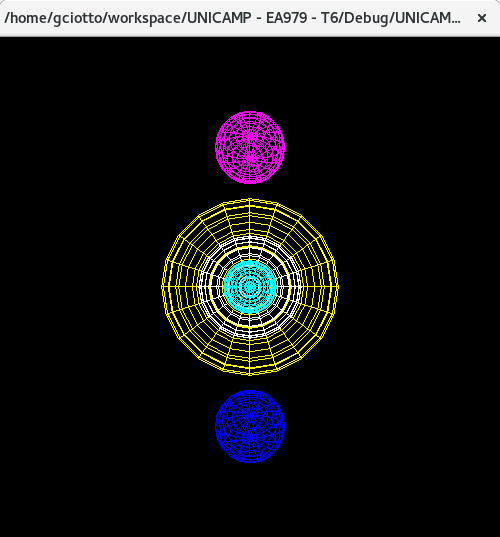
\includegraphics[scale=0.4]{init}
    \caption {Janela obtida após lançamento do programa.}
    \label{fig:inicializacao}
\end{figure} 

\FloatBarrier

Por fim, a documentação das funções nos aconselha a englobar todas as
tranformações \textit{model-view} dentro de um bloco \path{glPushMatrix()} -
\path{glPopMatrix()}, a fim de preservarmos o sistema de coordenadas anterior à
realização das operações.

\vspace{12pt}

A última etapa consistiu na rotação das esferas pela função \path{glRotatef}.
Além da rotação em torno do eixo \textbf{X}, já fornecido no modelo, adicionei
também a rotação ao redor do eixo \textbf{Y}. Para isso, criei uma nova variável
global, chamada de \path{cameraX}, que é incrementada/decrementada a cada
pressionamento da tecla \textit{X}/\textit{x} do teclado na função
\texttt{keyboard()}. O trecho abaixo, adicionado logo antes dos comandos que desenham as esferas, representa tal
funcionalidade:

\begin{lstlisting}[keywordstyle=\ttfamily, style=nonumbers]
glRotatef ((GLfloat) camera, 1.0, 0.0, 0.0);  /* Roda em torno de X */
glRotatef ((GLfloat) cameraX, 0.0, 1.0, 0.0); /* Roda em torno de Y */
\end{lstlisting}

As figuras abaixo representam algumas rotações realizadas pelo programa.

	\FloatBarrier
			    
	\begin{figure}[h!]
	
	\centering
	
		\begin{subfigure}{.33\textwidth}
		  \centering
		  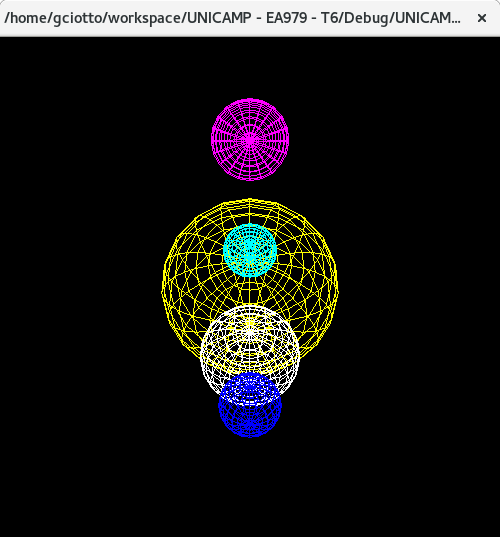
\includegraphics[scale=0.35]{ex1}
		  \caption{\centering Exemplo 1.}
		  
		\end{subfigure}%
		\begin{subfigure}{.33\textwidth}
		  \centering
		  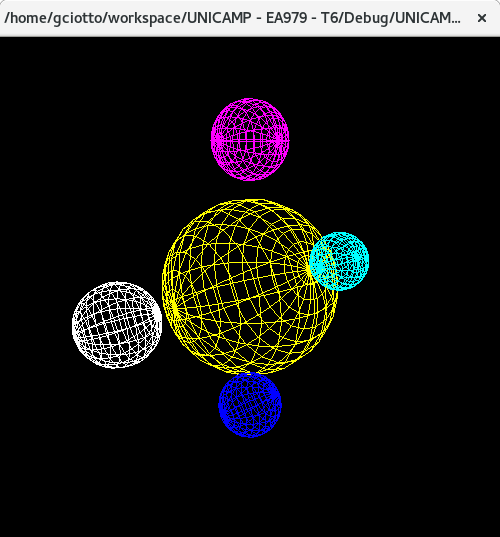
\includegraphics[scale=0.35]{ex2}
		  \caption{\centering Exemplo 2.}
		\end{subfigure}
		\begin{subfigure}{.33\textwidth}
		  \centering
		  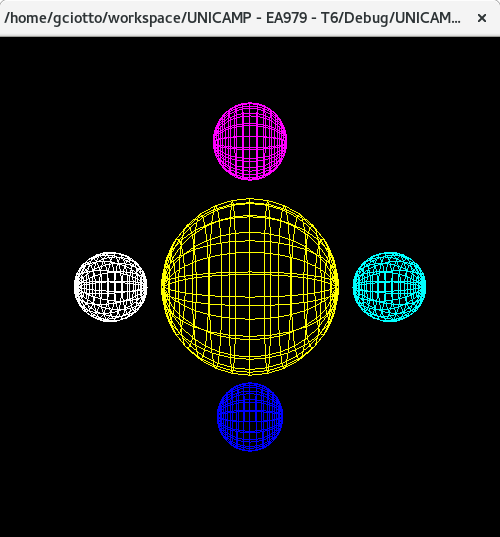
\includegraphics[scale=0.35]{ex3}
		  \caption{\centering Exemplo 3.} 
		\end{subfigure}
	
	
	\caption{Exemplos da execução do programa.}
	\end{figure} 
	
	\FloatBarrier

 \section* {Referências}

\begin {enumerate}
  \item 
  \textit  {What exactly are eye space coordinates?}, disponível em
  \url{http://stackoverflow.com/questions/15588860/what-exactly-are-eye-space-coordinates}.
  \end{enumerate}

\end{document}
